\documentclass[12pt,onecolumn]{article}
\usepackage[utf8]{inputenc} % UTF8 input encoding
\usepackage[T2A]{fontenc}   % T2A font encoding for Cyrillic script
\usepackage[russian]{babel} % Russian language support
\usepackage{listings}
\usepackage{float}
\usepackage{mathtools}
\everymath{\displaystyle}
\usepackage{listings} 
\usepackage[usenames]{color}
\usepackage{geometry}
\usepackage{verbatim}
\usepackage{tabularray}
\usepackage{color}
\newcommand{\nparagraph}[1]{\paragraph{#1}\mbox{}\\}
\geometry{
  a4paper,
  top=20mm, 
  right=25mm, 
  bottom=20mm, 
  left=20mm
}

\begin{document}
\setcounter{tocdepth}{4}
\begin{center}
    Федеральное государственное автономное образовательное учреждение высшего образования "Национальный Исследовательский Университет ИТМО"\\ 
    Мегафакультет Компьютерных Технологий и Управления\\
    Факультет Программной Инженерии и Компьютерной Техники \\
    
\includegraphics[scale=0.3]{image/itmo.jpg} % нужно закинуть картинку логтипа в папку с отчетом
\end{center}
\vspace{1cm}


\begin{center}
    \textbf{Домашнее задание 1}\\
    по дисциплине\\
    \textbf{Компьютерные сети}
\end{center}

\vspace{2cm}

\begin{flushright}
  Выполнил Студент  группы P33102\\
  \textbf{Лапин Алексей Александрович}\\
  Преподаватель: \\
  \textbf{Авксентьева Елена Юрьевна}\\
\end{flushright}

\vspace{6cm}
\begin{center}
    г. Санкт-Петербург\\
    2023г.
\end{center}

\newpage
\tableofcontents
\newpage

\section*{Цель работы:}
Изучение методов физического и логического кодирования, используемых в цифровых сетях передачи данных и исследование влияния свойств канала связи на качество передачи сигналов при различных методах физического и логического кодирования.
\section{Часть 1. Методы физического и логического кодирования}
\subsection{Этап 1. Формирование сообщения}
исходное сообщение: Лапин Алексей Александрович\\
в шестнадцатеричном коде: \\
CB E0 EF E8 ED 20\\
C0 EB E5 EA F1 E5 E9 20\\
C0 EB E5 EA F1 E0 ED E4 F0 EE E2 E8 F7\\
в двоичном коде:
\begin{verbatim}
Л cb 11001011
а e0 11100000
п ef 11101111
и e8 11101000
н ed 11101101
  20 00100000
А c0 11000000
л eb 11101011
е e5 11100101
к ea 11101010
с f1 11110001
е e5 11100101
й e9 11101001
  20 00100000
А c0 11000000
л eb 11101011
е e5 11100101
к ea 11101010
с f1 11110001
а e0 11100000
н ed 11101101
д e4 11100100
р f0 11110000
о ee 11101110
в e2 11100010
и e8 11101000
ч f7 11110111
\end{verbatim}
длина сообщения: 27 байт (216 бит)

\subsection{Этап 2. Физическое кодирование исходного сообщения}
\begin{figure}[H]
    \centering
    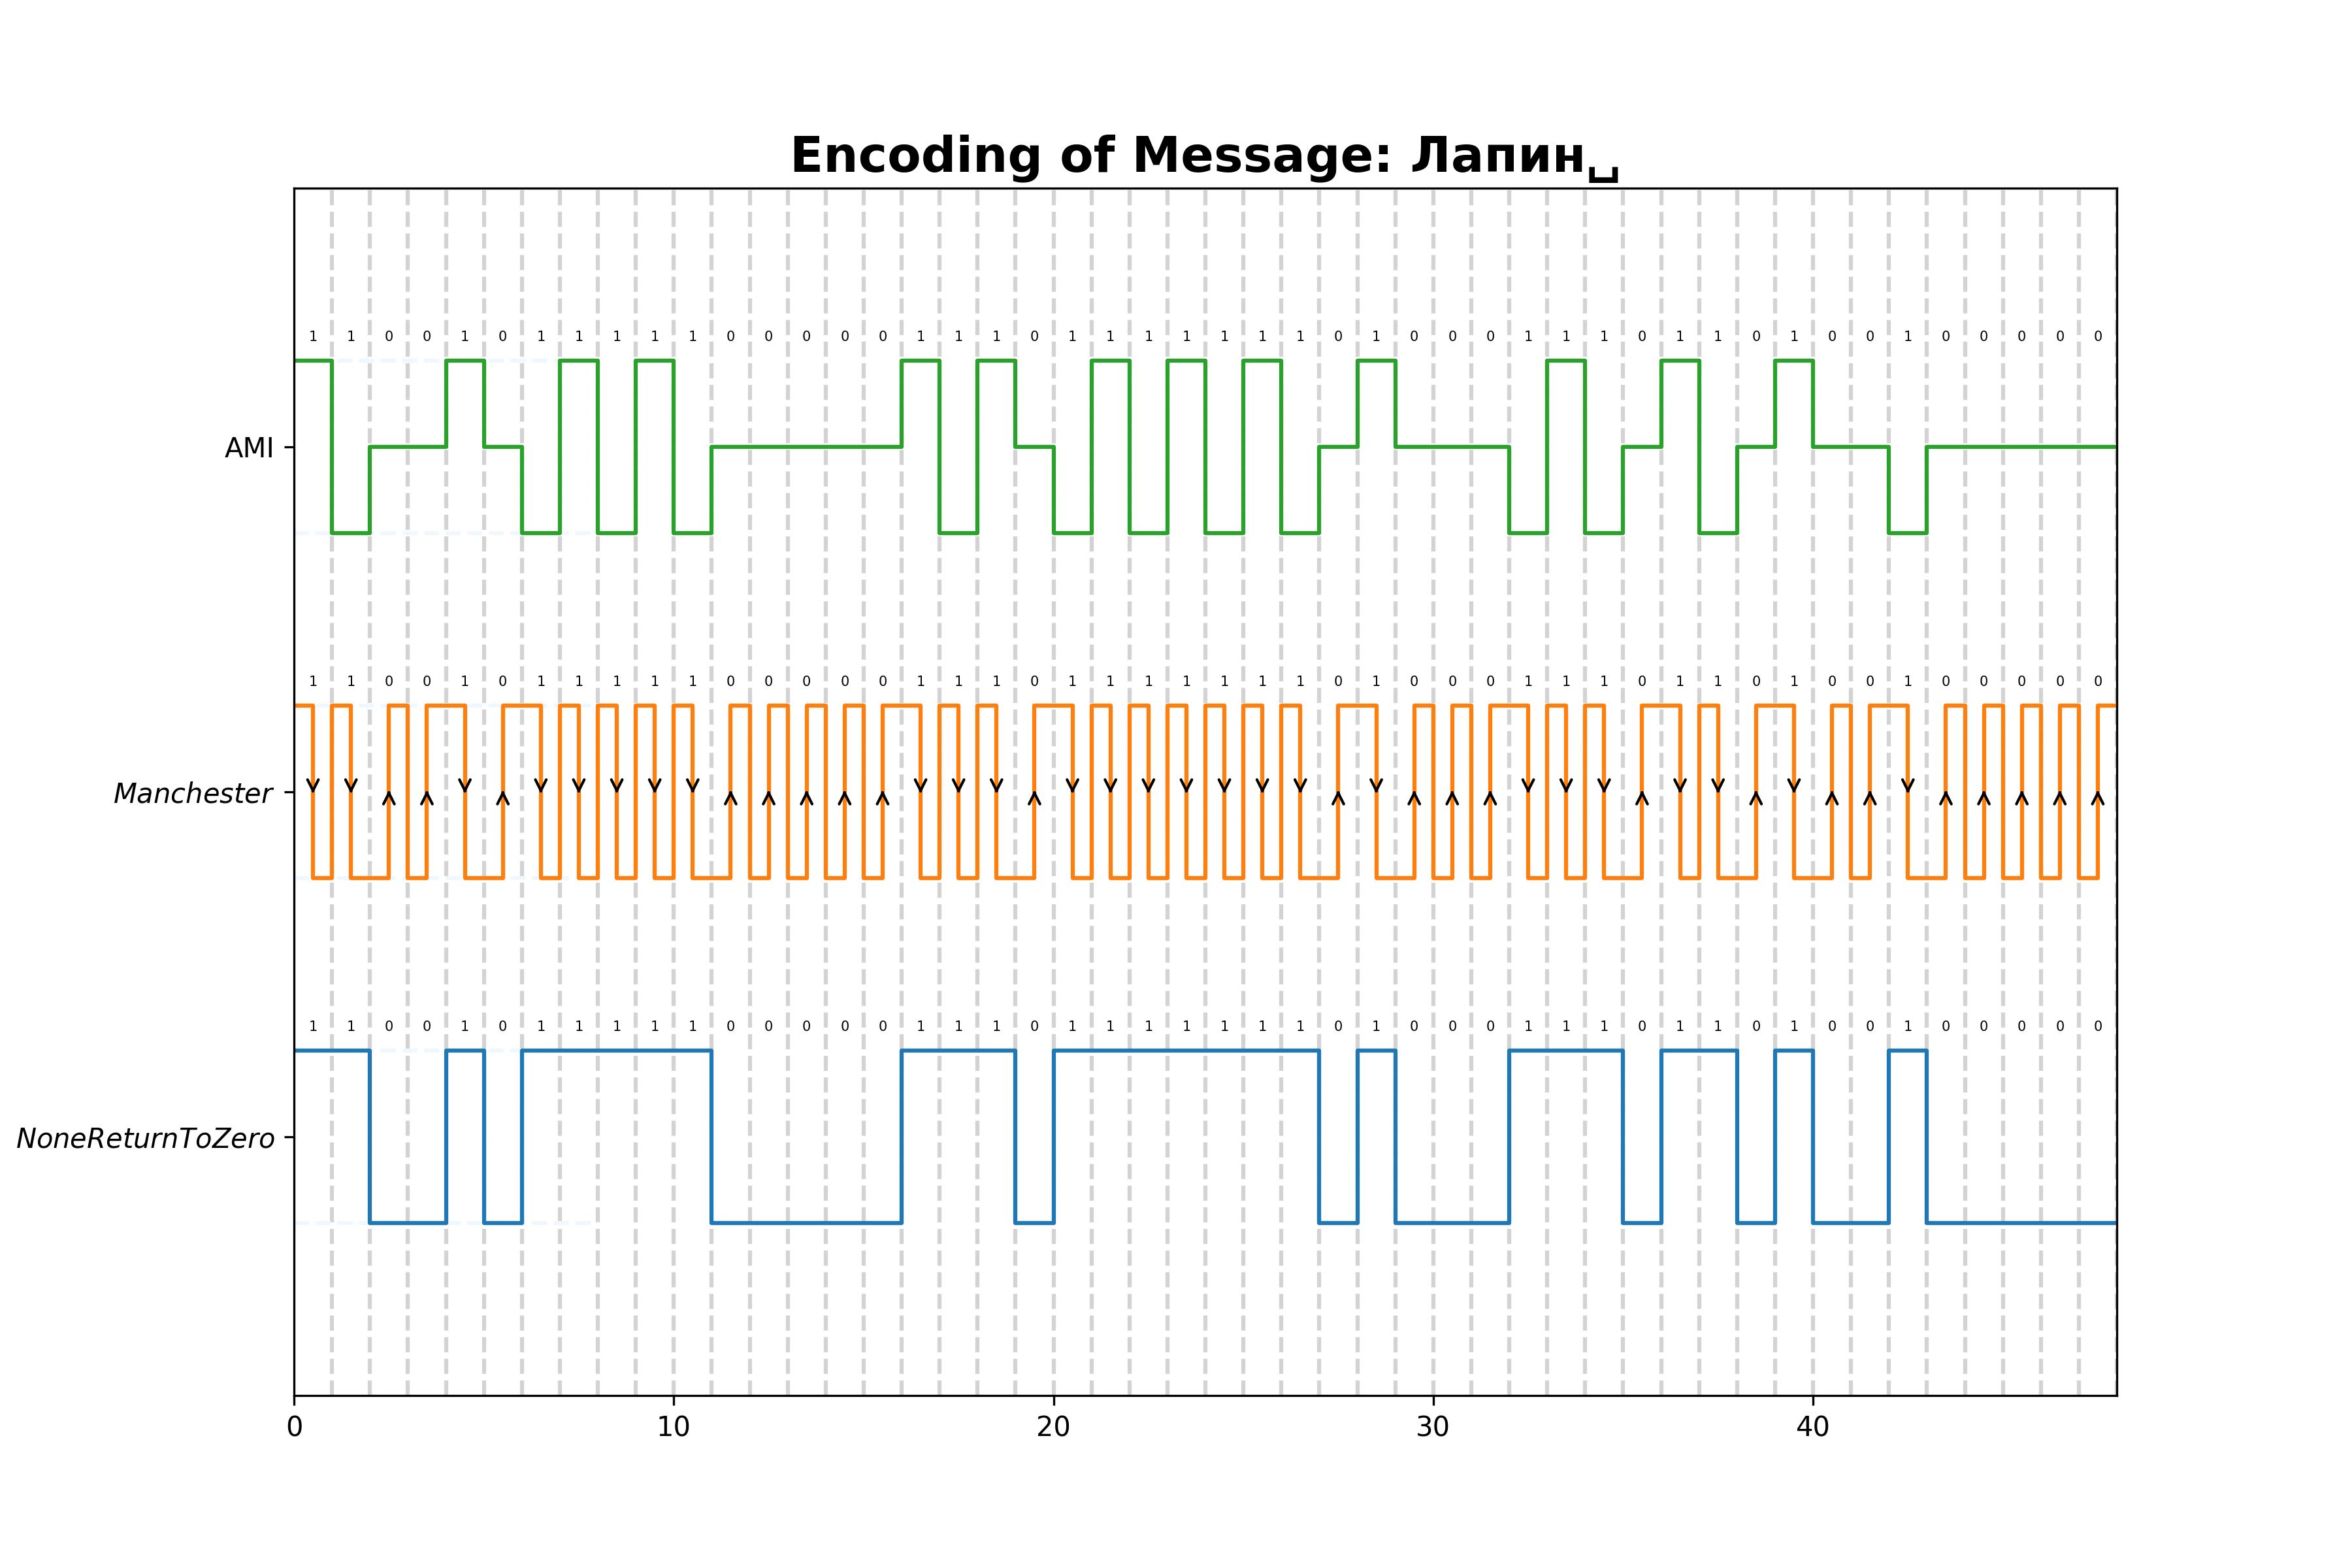
\includegraphics[width=\textwidth]{image/encoding_1.png}
    \caption{Физическое кодирование первой части сообщения}
\end{figure}
\begin{figure}[H]
    \centering
    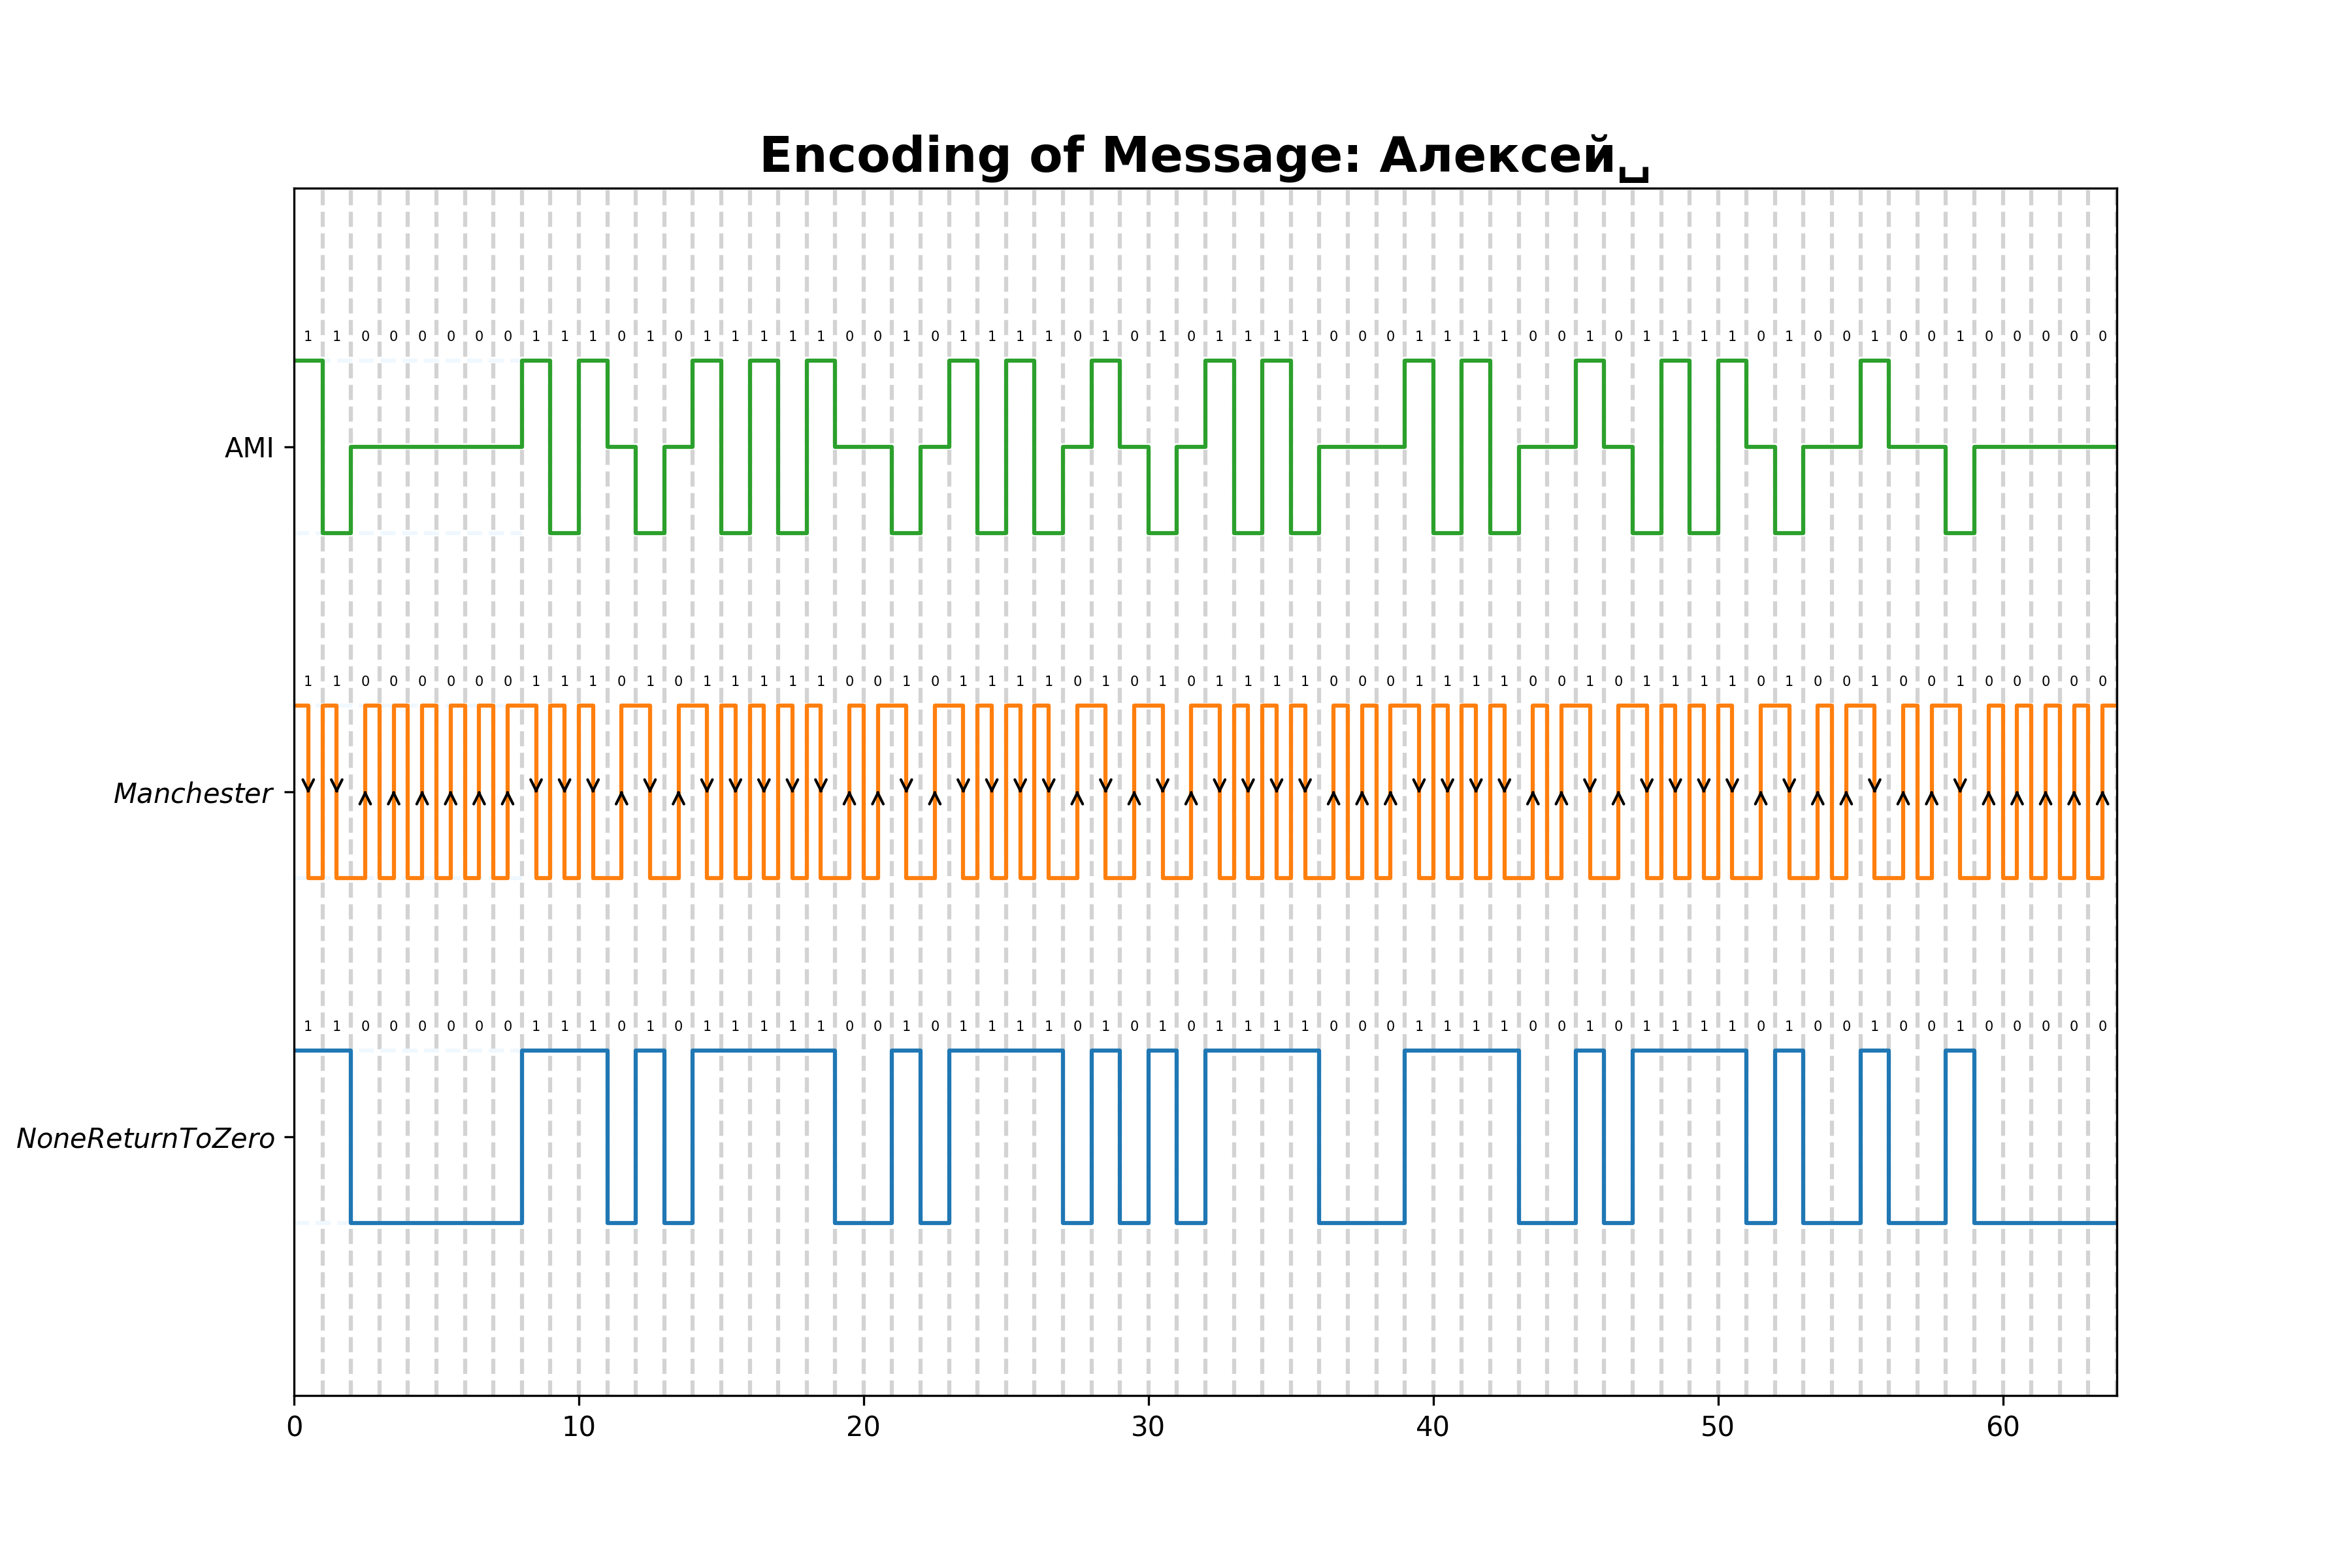
\includegraphics[width=\textwidth]{image/encoding_2.png}
    \caption{Физическое кодирование второй части сообщения}
\end{figure}
\begin{figure}[H]
    \centering
    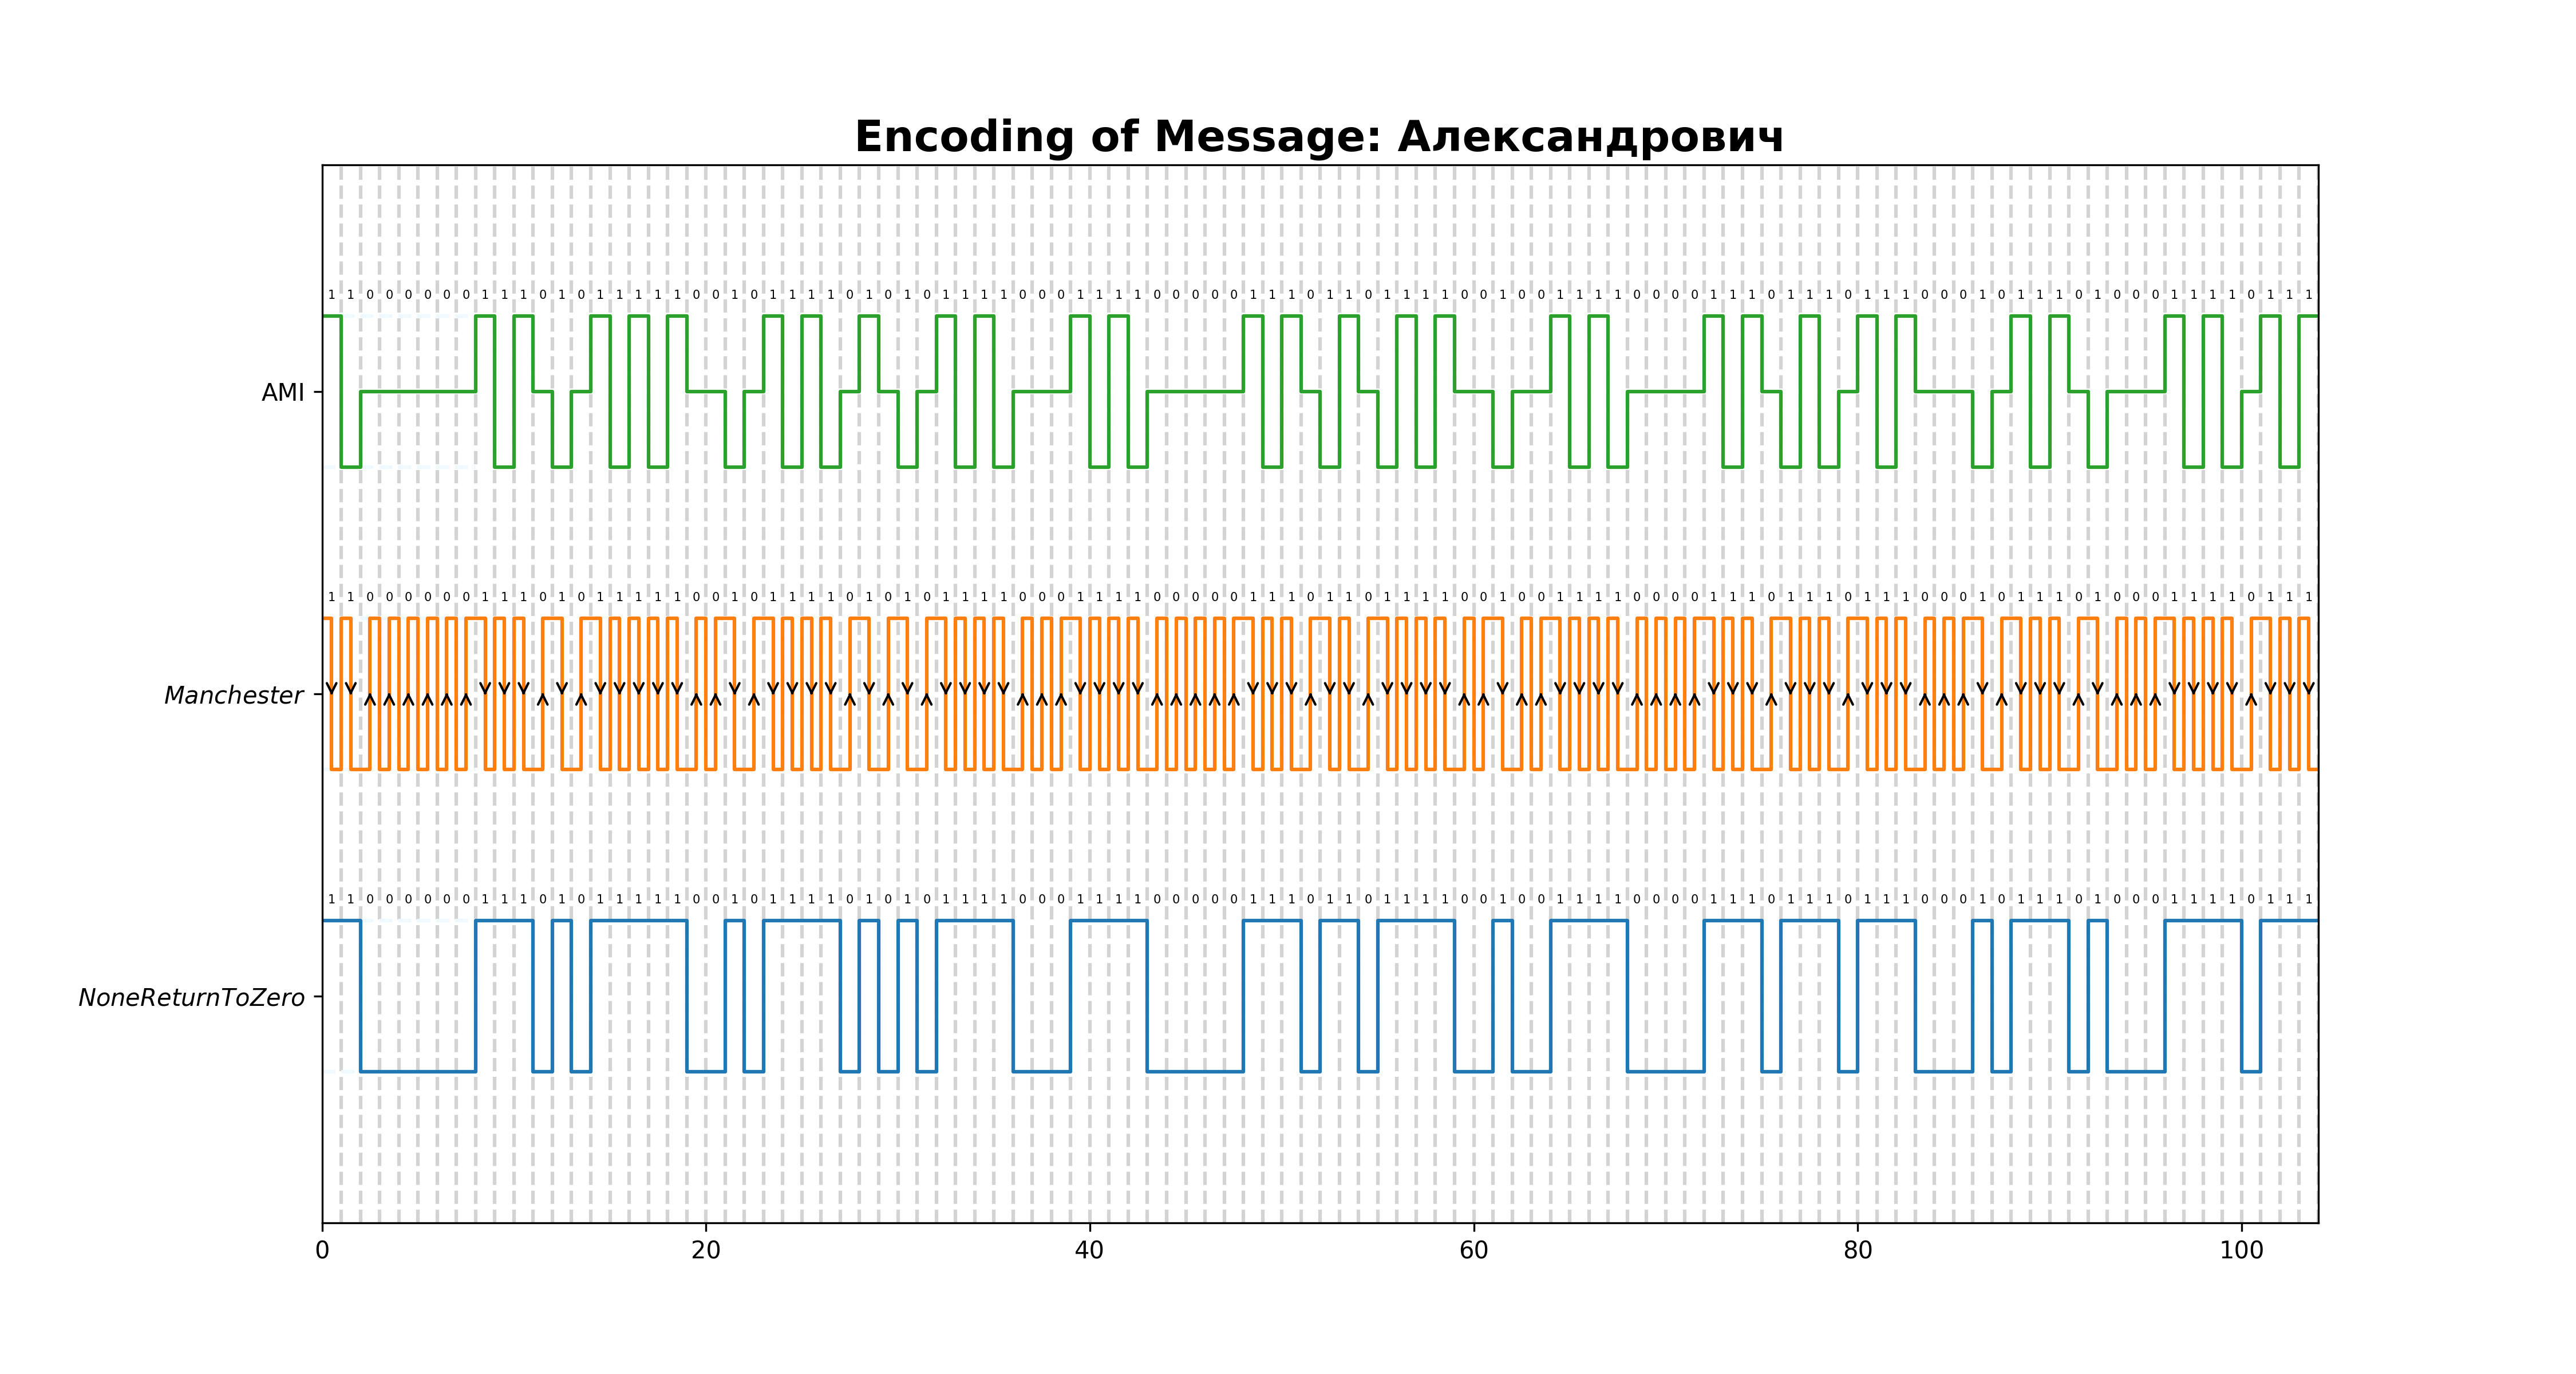
\includegraphics[width=\textwidth]{image/encoding_3.png}
    \caption{Физическое кодирование третьей части сообщения}
\end{figure}
\subsubsection{Манчестерский код}
Верхняя граница частот: $f_{\text{в}} = C = 100~ \text{МГц}$\\
Нижняя граница частот: $f_{\text{н}} = \frac{C}{2} = 50~ \text{МГц}$\\
Спектр сигнала: $S = f_{\text{в}} - f_{\text{н}} = 100 - 50 = 50~\text{МГц}$\\
Среднее значение частоты: $f_{\text{ср}} =  \frac{244\cdot f_0 + 188 \cdot \frac{f_0}{2}}{432} \approx 78.24~\text{МГц}$\\
Середина спектра: $f_{1/2} = \frac{f_{\text{в}} + f_{\text{н}}}{2} = \frac{100 + 50}{2} = 75~\text{МГц}$\\
Спектр сигнала: $S = 7\cdot f_0 - \frac{f_0}{2} = 100 \cdot (7 - 0.5)= 650~\text{МГц}$\\
Полоса пропускания: $F = 650~ \text{МГц}$
\subsubsection{NRZ код}
Fundamental frequency: $f_{\text{0}} = \frac{C}{2} = \frac{100}{2} = 50~\text{МГц}$\\
Верхняя граница частот: $T = 2t, ~t = \frac{1}{C} \to f_{\text{в}} = \frac{1}{T} = \frac{C}{2} = 50~\text{МГц}$\\
Нижняя граница частот: $f_{\text{н}} = \frac{f_{\text{0}}}{7} = \frac{50}{7} \approx 7.143~\text{МГц}$\\
Спектр сигнала: $S = f_{\text{в}} - f_{\text{н}} = 50 - 7.143 = 42.857 ~\text{МГц}$\\
Среднее значение частоты: $f_{\text{ср}} = \frac{45\cdot f_0 + 28 \cdot \frac{f_0}{2} + 45 \cdot \frac{f_0}{3} + 44 \cdot \frac{f_0}{4} + 35 \cdot \frac{f_0}{5} + 12 \cdot \frac{f_0}{6} + 7 \cdot \frac{f_0}{7}}{216} \approx 21.99~\text{МГц}$\\
Середина спектра: $f_{1/2} = \frac{f_{\text{в}} + f_{\text{н}}}{2} = \frac{50 + 7.143}{2} = 28.571~\text{МГц}$\\
Спектр сигнала: $S = 7\cdot f_0 - \frac{f_0}{7} = 50 \cdot \left(7 -\frac{1}{7}\right) = 342.857 ~\text{МГц}$\\
Полоса пропускания: $F = 343~ \text{МГц}$
\subsubsection{AMI код}
Fundamental frequency: $f_{\text{0}} = \frac{C}{2} = \frac{100}{2} = 50~\text{МГц}$\\
Верхняя граница частот: $T = 2t, ~t = \frac{1}{C} \to f_{\text{в}} = \frac{1}{T} = \frac{C}{2} = 50~\text{МГц}$\\
Нижняя граница частот: $f_{\text{н}} = \frac{f_{\text{0}}}{6} = \frac{50}{6} \approx 8.334~\text{МГц}$\\
Спектр сигнала: $S = f_{\text{в}} - f_{\text{н}} = 50 - 8.334 = 41.666 ~\text{МГц}$\\
Среднее значение частоты: $f_{\text{ср}} = \frac{147\cdot f_0 + 18 \cdot \frac{f_0}{2} + 15 \cdot \frac{f_0}{3} + 4 \cdot \frac{f_0}{4} + 20 \cdot \frac{f_0}{5} + 12 \cdot \frac{f_0}{6}}{216} \approx 38.889~\text{МГц}$\\
Середина спектра: $f_{1/2} = \frac{f_{\text{в}} + f_{\text{н}}}{2} = \frac{50 + 8.334}{2} = 29.167~\text{МГц}$\\
Спектр сигнала: $S = 7\cdot f_0 - \frac{f_0}{6} = 50 \cdot \left(7 -\frac{1}{6}\right) = 341.667 ~\text{МГц}$\\
Полоса пропускания: $F = 342~ \text{МГц}$

\definecolor{Cinnabar}{rgb}{0.917,0.262,0.207}
\definecolor{ChateauGreen}{rgb}{0.203,0.658,0.325}
\definecolor{SelectiveYellow}{rgb}{0.984,0.737,0.015}
\begin{longtblr}[
  label = none,
  entry = none,
]{
  width = \linewidth,
  colspec = {Q[146]Q[167]Q[113]Q[188]Q[156]Q[163]},
  cells = {c},
  cell{2}{2} = {Cinnabar},
  cell{2}{3} = {ChateauGreen},
  cell{2}{4} = {ChateauGreen},
  cell{2}{5} = {ChateauGreen},
  cell{2}{6} = {SelectiveYellow},
  cell{3}{2} = {ChateauGreen},
  cell{3}{3} = {Cinnabar},
  cell{3}{4} = {Cinnabar},
  cell{3}{5} = {Cinnabar},
  cell{3}{6} = {ChateauGreen},
  cell{4}{2} = {ChateauGreen},
  cell{4}{3} = {Cinnabar},
  cell{4}{4} = {Cinnabar},
  cell{4}{5} = {ChateauGreen},
  cell{4}{6} = {Cinnabar},
  hlines,
  vlines,
}
Метод кодирования & Спектор сигнала (МГц) & Само синхронизация & Постоянная составляющая & Обнаружение ошибок & Стоимость реализации \\
M2                & 50                   & есть                  & нет                     & есть               & 2                    \\
NRZ               & 43                   & нет                   & есть                    & нет                & 1                    \\
AMI               & 42                   & нет                   & есть                    & есть               & 3                    
\end{longtblr}

В результате сравения можно сделать вывод, что лучшим способом кодирования является M2. Он обладает самосинхронизацией, обнаружением ошибок, требует всего два уровня сигнала и не имеет постоянной составляющей.
Однако есть и недостаток в большем спекторе сигнала по сравнению с NRZ и AMI.

На втором месте, я бы взял AMI, так как он обладает обнаружением ошибок и самым маленьким спектром сигнала.
\subsection{Этап 3. Логическое (избыточное) кодирование исходного сообщения}
\begin{verbatim}
1100 -> 11010
1001 -> 10111
0010 -> 11100
0101 -> 11110
1011 -> 11100
0111 -> 11101
1111 -> 11100
1111 -> 10010
1110 -> 11100
1100 -> 11011
1000 -> 10100
0000 -> 11110
0000 -> 11010
0001 -> 11110
0011 -> 11100
0111 -> 10111
1110 -> 11100
1101 -> 01011
1011 -> 11100
0111 -> 10110
1111 -> 11101
1111 -> 01001
1111 -> 11100
1111 -> 01011
1110 -> 11100
1101 -> 10011
1010 -> 10100
0100 -> 11110
1000 -> 11010
0001 -> 11110
0011 -> 11100
0111 -> 10111
1110 -> 11100
1101 -> 01011
1011 -> 11100
0110 -> 10110
1101 -> 11101
1010 -> 01001
0100 -> 11100
1001 -> 11110
0010 -> 11100
0100 -> 11011
1000 -> 11100
0000 -> 01010
0000 -> 11101
0001 -> 11110
0011 -> 11100
0110 -> 11100
1100 -> 11100
1000 -> 10100
0000 -> 11100
0000 -> 10010
0000 -> 11101
0001 -> 01111
\end{verbatim}
В двоичном коде: 110101011111100111101110011101111001001011100110111010011110\\
110101111011100101111110001011111001011011101010011110001011\\
111001001110100111101101011110111001011111100010111110010110\\
111010100111100111101110011011111000101011101111101110011100\\
111001010011100100101110101111\\
В шестнадцатеричном коде: 0x357e7b9de4b9ba7b5ee5f8be5ba9e2f93a7b5ee5f8be5ba9\\
e7b9be2bbee7394e4baf\\
Длина сообщения: 33.75 байт (270 бит)\\
Избыточность: 25\%
\begin{figure}[H]
    \centering
    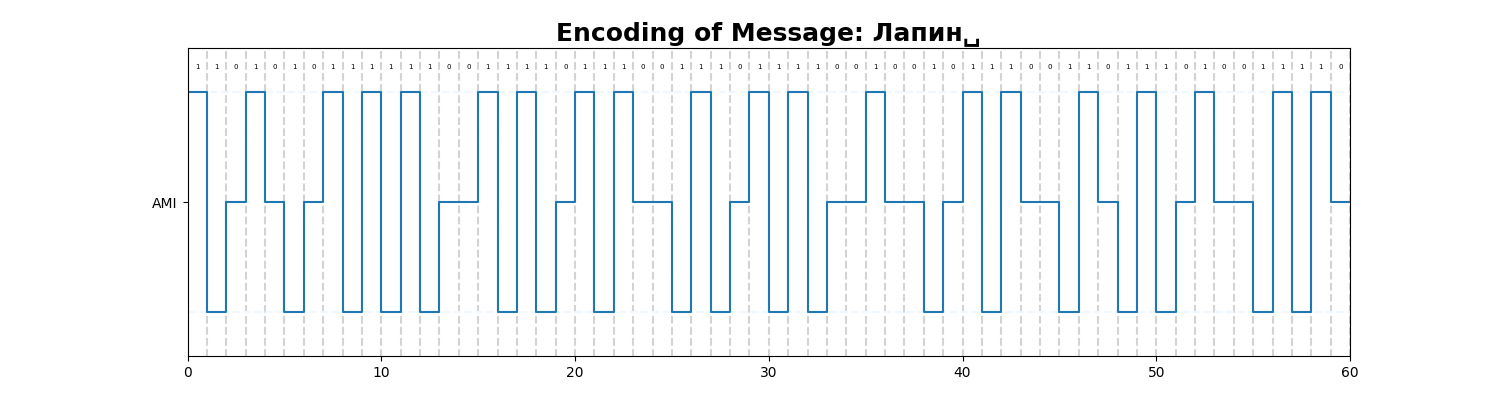
\includegraphics[width=\textwidth]{image/encoding_2-1.png}
    \caption{Логическое кодирование 4B/5B сообщения}
\end{figure}
\begin{figure}[H]
    \centering
    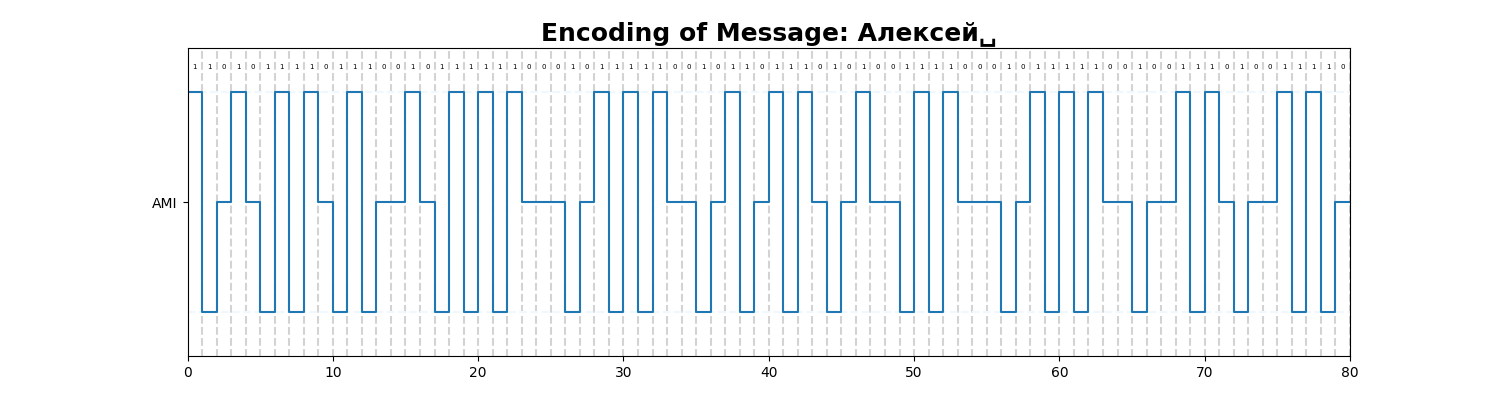
\includegraphics[width=\textwidth]{image/encoding_2-2.png}
    \caption{Логическое кодирование 4B/5B сообщения}
\end{figure}
\begin{figure}[H]
    \centering
    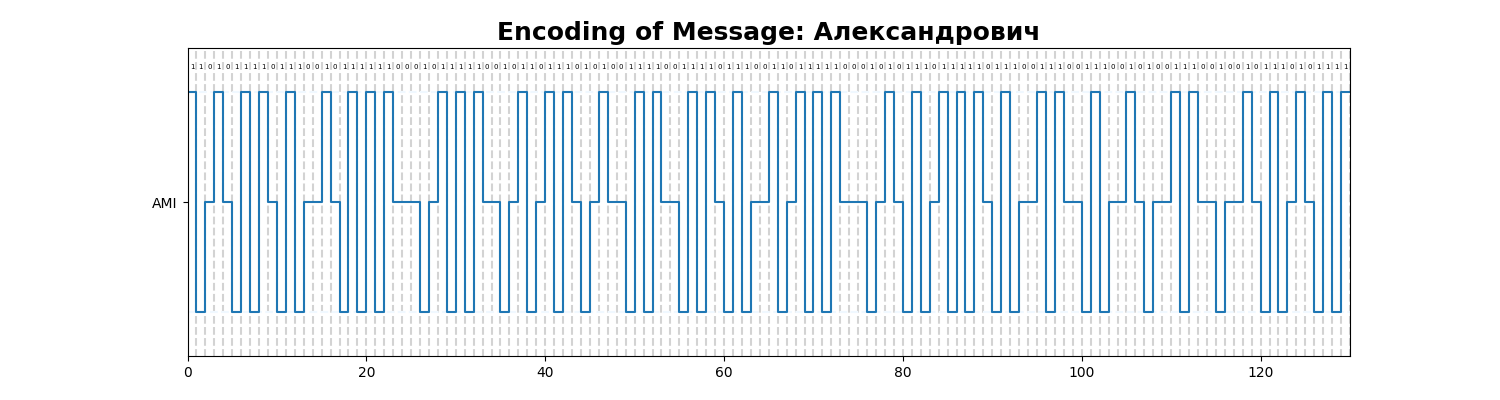
\includegraphics[width=\textwidth]{image/encoding_2-3.png}
    \caption{Логическое кодирование 4B/5B сообщения}
\end{figure}

Верхняя граница частот: $f_{\text{в}} = \frac{C}{2} = 50~ \text{МГц}$

Нижняя граница частот: $f_{\text{н}} = \frac{f_0}{3} = 16.67 ~ \text{МГц}$

Средняя частота: $f_{\text{ср}} = \frac{212\cdot f_0 + 23\cdot 2\cdot \frac{f_0}{2} + 4\cdot3 \cdot \frac{f_0}{3}}{270} \approx 44.259~\text{МГц}$

Середина спектра: $f_{1/2} = \frac{f_{\text{в}} + f_{\text{н}}}{2} = \frac{50 + 16.67}{2} = 33.335~\text{МГц}$

Спектр сигнала: $S = f_{\text{в}} - f_{\text{н}} = 50 - 16.67 = 33.33~\text{МГц}$

Полоса пропускания: $F = 34~ \text{МГц}$

Сравнивая с результами физичекого кодирования AMI кода, мы видим, что спектр сигнала сузился. Также логическое кодирование 4B/5B дало коду возможность обнаружения ошибки и самосинхронизацию.



\subsection{Этап 4. Скремблирование исходного сообщения}
$$B_i = A_i \oplus B_{i-1} \oplus B_{i-15}$$

Выбран этот полином, так как он выдает наименьшую длинну постоянной (повторяющихся нулей). Это было проверено перебором всех возможных полиномов.\\
Максимальная длина повторяющихся нулей: 4.

$$B_{1} = A_{1}= 1$$
$$B_{2} = A_{2}= 1$$
$$B_{3} = A_{3}= 0$$
$$B_{4} = A_{4}= 0$$
$$B_{5} = A_{5}= 1$$
$$B_{6} = A_{6}= 0$$
$$B_{7} = A_{7}= 1$$
$$B_{8} = A_{8}= 1$$
$$B_{9} = A_{9}= 1$$
$$B_{10} = A_{10}= 1$$
$$B_{11} = A_{11}= 1$$
$$B_{12} = A_{12}= 0$$
$$B_{13} = A_{13}= 0$$
$$B_{14} = A_{14}= 0$$
$$B_{15} = A_{15}= 0$$
$$B_{16} = A_{16} \oplus B_{1} = 0 \oplus 1 = 1$$
$$B_{17} = A_{17} \oplus B_{2} \oplus B_{1} = 1 \oplus 1 \oplus 1 = 1$$
$$B_{18} = A_{18} \oplus B_{3} \oplus B_{2} = 1 \oplus 0 \oplus 1 = 0$$
$$B_{19} = A_{19} \oplus B_{4} \oplus B_{3} = 1 \oplus 0 \oplus 0 = 1$$
$$B_{20} = A_{20} \oplus B_{5} \oplus B_{4} = 0 \oplus 1 \oplus 0 = 1$$
$$B_{21} = A_{21} \oplus B_{6} \oplus B_{5} = 1 \oplus 0 \oplus 1 = 0$$
$$B_{22} = A_{22} \oplus B_{7} \oplus B_{6} = 1 \oplus 1 \oplus 0 = 0$$
$$B_{23} = A_{23} \oplus B_{8} \oplus B_{7} = 1 \oplus 1 \oplus 1 = 1$$
$$B_{24} = A_{24} \oplus B_{9} \oplus B_{8} = 1 \oplus 1 \oplus 1 = 1$$
$$B_{25} = A_{25} \oplus B_{10} \oplus B_{9} = 1 \oplus 1 \oplus 1 = 1$$
$$B_{26} = A_{26} \oplus B_{11} \oplus B_{10} = 1 \oplus 1 \oplus 1 = 1$$
$$B_{27} = A_{27} \oplus B_{12} \oplus B_{11} = 1 \oplus 0 \oplus 1 = 0$$
$$B_{28} = A_{28} \oplus B_{13} \oplus B_{12} = 0 \oplus 0 \oplus 0 = 0$$
$$B_{29} = A_{29} \oplus B_{14} \oplus B_{13} = 1 \oplus 0 \oplus 0 = 1$$
$$B_{30} = A_{30} \oplus B_{15} \oplus B_{14} = 0 \oplus 0 \oplus 0 = 0$$
$$B_{31} = A_{31} \oplus B_{16} \oplus B_{15} = 0 \oplus 1 \oplus 0 = 1$$
$$B_{32} = A_{32} \oplus B_{17} \oplus B_{16} = 0 \oplus 1 \oplus 1 = 0$$
$$B_{33} = A_{33} \oplus B_{18} \oplus B_{17} = 1 \oplus 0 \oplus 1 = 0$$
$$B_{34} = A_{34} \oplus B_{19} \oplus B_{18} = 1 \oplus 1 \oplus 0 = 0$$
$$B_{35} = A_{35} \oplus B_{20} \oplus B_{19} = 1 \oplus 1 \oplus 1 = 1$$
$$B_{36} = A_{36} \oplus B_{21} \oplus B_{20} = 0 \oplus 0 \oplus 1 = 1$$
$$B_{37} = A_{37} \oplus B_{22} \oplus B_{21} = 1 \oplus 0 \oplus 0 = 1$$
$$B_{38} = A_{38} \oplus B_{23} \oplus B_{22} = 1 \oplus 1 \oplus 0 = 0$$
$$B_{39} = A_{39} \oplus B_{24} \oplus B_{23} = 0 \oplus 1 \oplus 1 = 0$$
$$B_{40} = A_{40} \oplus B_{25} \oplus B_{24} = 1 \oplus 1 \oplus 1 = 1$$
$$B_{41} = A_{41} \oplus B_{26} \oplus B_{25} = 0 \oplus 1 \oplus 1 = 0$$
$$B_{42} = A_{42} \oplus B_{27} \oplus B_{26} = 0 \oplus 0 \oplus 1 = 1$$
$$B_{43} = A_{43} \oplus B_{28} \oplus B_{27} = 1 \oplus 0 \oplus 0 = 1$$
$$B_{44} = A_{44} \oplus B_{29} \oplus B_{28} = 0 \oplus 1 \oplus 0 = 1$$
$$B_{45} = A_{45} \oplus B_{30} \oplus B_{29} = 0 \oplus 0 \oplus 1 = 1$$
$$B_{46} = A_{46} \oplus B_{31} \oplus B_{30} = 0 \oplus 1 \oplus 0 = 1$$
$$B_{47} = A_{47} \oplus B_{32} \oplus B_{31} = 0 \oplus 0 \oplus 1 = 1$$
$$B_{48} = A_{48} \oplus B_{33} \oplus B_{32} = 0 \oplus 0 \oplus 0 = 0$$
$$B_{49} = A_{49} \oplus B_{34} \oplus B_{33} = 1 \oplus 0 \oplus 0 = 1$$
$$B_{50} = A_{50} \oplus B_{35} \oplus B_{34} = 1 \oplus 1 \oplus 0 = 0$$
$$B_{51} = A_{51} \oplus B_{36} \oplus B_{35} = 0 \oplus 1 \oplus 1 = 0$$
$$B_{52} = A_{52} \oplus B_{37} \oplus B_{36} = 0 \oplus 1 \oplus 1 = 0$$
$$B_{53} = A_{53} \oplus B_{38} \oplus B_{37} = 0 \oplus 0 \oplus 1 = 1$$
$$B_{54} = A_{54} \oplus B_{39} \oplus B_{38} = 0 \oplus 0 \oplus 0 = 0$$
$$B_{55} = A_{55} \oplus B_{40} \oplus B_{39} = 0 \oplus 1 \oplus 0 = 1$$
$$B_{56} = A_{56} \oplus B_{41} \oplus B_{40} = 0 \oplus 0 \oplus 1 = 1$$
$$B_{57} = A_{57} \oplus B_{42} \oplus B_{41} = 1 \oplus 1 \oplus 0 = 0$$
$$B_{58} = A_{58} \oplus B_{43} \oplus B_{42} = 1 \oplus 1 \oplus 1 = 1$$
$$B_{59} = A_{59} \oplus B_{44} \oplus B_{43} = 1 \oplus 1 \oplus 1 = 1$$
$$B_{60} = A_{60} \oplus B_{45} \oplus B_{44} = 0 \oplus 1 \oplus 1 = 0$$
$$B_{61} = A_{61} \oplus B_{46} \oplus B_{45} = 1 \oplus 1 \oplus 1 = 1$$
$$B_{62} = A_{62} \oplus B_{47} \oplus B_{46} = 0 \oplus 1 \oplus 1 = 0$$
$$B_{63} = A_{63} \oplus B_{48} \oplus B_{47} = 1 \oplus 0 \oplus 1 = 0$$
$$B_{64} = A_{64} \oplus B_{49} \oplus B_{48} = 1 \oplus 1 \oplus 0 = 0$$
$$B_{65} = A_{65} \oplus B_{50} \oplus B_{49} = 1 \oplus 0 \oplus 1 = 0$$
$$B_{66} = A_{66} \oplus B_{51} \oplus B_{50} = 1 \oplus 0 \oplus 0 = 1$$
$$B_{67} = A_{67} \oplus B_{52} \oplus B_{51} = 1 \oplus 0 \oplus 0 = 1$$
$$B_{68} = A_{68} \oplus B_{53} \oplus B_{52} = 0 \oplus 1 \oplus 0 = 1$$
$$B_{69} = A_{69} \oplus B_{54} \oplus B_{53} = 0 \oplus 0 \oplus 1 = 1$$
$$B_{70} = A_{70} \oplus B_{55} \oplus B_{54} = 1 \oplus 1 \oplus 0 = 0$$
$$B_{71} = A_{71} \oplus B_{56} \oplus B_{55} = 0 \oplus 1 \oplus 1 = 0$$
$$B_{72} = A_{72} \oplus B_{57} \oplus B_{56} = 1 \oplus 0 \oplus 1 = 0$$
$$B_{73} = A_{73} \oplus B_{58} \oplus B_{57} = 1 \oplus 1 \oplus 0 = 0$$
$$B_{74} = A_{74} \oplus B_{59} \oplus B_{58} = 1 \oplus 1 \oplus 1 = 1$$
$$B_{75} = A_{75} \oplus B_{60} \oplus B_{59} = 1 \oplus 0 \oplus 1 = 0$$
$$B_{76} = A_{76} \oplus B_{61} \oplus B_{60} = 0 \oplus 1 \oplus 0 = 1$$
$$B_{77} = A_{77} \oplus B_{62} \oplus B_{61} = 1 \oplus 0 \oplus 1 = 0$$
$$B_{78} = A_{78} \oplus B_{63} \oplus B_{62} = 0 \oplus 0 \oplus 0 = 0$$
$$B_{79} = A_{79} \oplus B_{64} \oplus B_{63} = 1 \oplus 0 \oplus 0 = 1$$
$$B_{80} = A_{80} \oplus B_{65} \oplus B_{64} = 0 \oplus 0 \oplus 0 = 0$$
$$B_{81} = A_{81} \oplus B_{66} \oplus B_{65} = 1 \oplus 1 \oplus 0 = 0$$
$$B_{82} = A_{82} \oplus B_{67} \oplus B_{66} = 1 \oplus 1 \oplus 1 = 1$$
$$B_{83} = A_{83} \oplus B_{68} \oplus B_{67} = 1 \oplus 1 \oplus 1 = 1$$
$$B_{84} = A_{84} \oplus B_{69} \oplus B_{68} = 1 \oplus 1 \oplus 1 = 1$$
$$B_{85} = A_{85} \oplus B_{70} \oplus B_{69} = 0 \oplus 0 \oplus 1 = 1$$
$$B_{86} = A_{86} \oplus B_{71} \oplus B_{70} = 0 \oplus 0 \oplus 0 = 0$$
$$B_{87} = A_{87} \oplus B_{72} \oplus B_{71} = 0 \oplus 0 \oplus 0 = 0$$
$$B_{88} = A_{88} \oplus B_{73} \oplus B_{72} = 1 \oplus 0 \oplus 0 = 1$$
$$B_{89} = A_{89} \oplus B_{74} \oplus B_{73} = 1 \oplus 1 \oplus 0 = 0$$
$$B_{90} = A_{90} \oplus B_{75} \oplus B_{74} = 1 \oplus 0 \oplus 1 = 0$$
$$B_{91} = A_{91} \oplus B_{76} \oplus B_{75} = 1 \oplus 1 \oplus 0 = 0$$
$$B_{92} = A_{92} \oplus B_{77} \oplus B_{76} = 0 \oplus 0 \oplus 1 = 1$$
$$B_{93} = A_{93} \oplus B_{78} \oplus B_{77} = 0 \oplus 0 \oplus 0 = 0$$
$$B_{94} = A_{94} \oplus B_{79} \oplus B_{78} = 1 \oplus 1 \oplus 0 = 0$$
$$B_{95} = A_{95} \oplus B_{80} \oplus B_{79} = 0 \oplus 0 \oplus 1 = 1$$
$$B_{96} = A_{96} \oplus B_{81} \oplus B_{80} = 1 \oplus 0 \oplus 0 = 1$$
$$B_{97} = A_{97} \oplus B_{82} \oplus B_{81} = 1 \oplus 1 \oplus 0 = 0$$
$$B_{98} = A_{98} \oplus B_{83} \oplus B_{82} = 1 \oplus 1 \oplus 1 = 1$$
$$B_{99} = A_{99} \oplus B_{84} \oplus B_{83} = 1 \oplus 1 \oplus 1 = 1$$
$$B_{100} = A_{100} \oplus B_{85} \oplus B_{84} = 0 \oplus 1 \oplus 1 = 0$$
$$B_{101} = A_{101} \oplus B_{86} \oplus B_{85} = 1 \oplus 0 \oplus 1 = 0$$
$$B_{102} = A_{102} \oplus B_{87} \oplus B_{86} = 0 \oplus 0 \oplus 0 = 0$$
$$B_{103} = A_{103} \oplus B_{88} \oplus B_{87} = 0 \oplus 1 \oplus 0 = 1$$
$$B_{104} = A_{104} \oplus B_{89} \oplus B_{88} = 1 \oplus 0 \oplus 1 = 0$$
$$B_{105} = A_{105} \oplus B_{90} \oplus B_{89} = 0 \oplus 0 \oplus 0 = 0$$
$$B_{106} = A_{106} \oplus B_{91} \oplus B_{90} = 0 \oplus 0 \oplus 0 = 0$$
$$B_{107} = A_{107} \oplus B_{92} \oplus B_{91} = 1 \oplus 1 \oplus 0 = 0$$
$$B_{108} = A_{108} \oplus B_{93} \oplus B_{92} = 0 \oplus 0 \oplus 1 = 1$$
$$B_{109} = A_{109} \oplus B_{94} \oplus B_{93} = 0 \oplus 0 \oplus 0 = 0$$
$$B_{110} = A_{110} \oplus B_{95} \oplus B_{94} = 0 \oplus 1 \oplus 0 = 1$$
$$B_{111} = A_{111} \oplus B_{96} \oplus B_{95} = 0 \oplus 1 \oplus 1 = 0$$
$$B_{112} = A_{112} \oplus B_{97} \oplus B_{96} = 0 \oplus 0 \oplus 1 = 1$$
$$B_{113} = A_{113} \oplus B_{98} \oplus B_{97} = 1 \oplus 1 \oplus 0 = 0$$
$$B_{114} = A_{114} \oplus B_{99} \oplus B_{98} = 1 \oplus 1 \oplus 1 = 1$$
$$B_{115} = A_{115} \oplus B_{100} \oplus B_{99} = 0 \oplus 0 \oplus 1 = 1$$
$$B_{116} = A_{116} \oplus B_{101} \oplus B_{100} = 0 \oplus 0 \oplus 0 = 0$$
$$B_{117} = A_{117} \oplus B_{102} \oplus B_{101} = 0 \oplus 0 \oplus 0 = 0$$
$$B_{118} = A_{118} \oplus B_{103} \oplus B_{102} = 0 \oplus 1 \oplus 0 = 1$$
$$B_{119} = A_{119} \oplus B_{104} \oplus B_{103} = 0 \oplus 0 \oplus 1 = 1$$
$$B_{120} = A_{120} \oplus B_{105} \oplus B_{104} = 0 \oplus 0 \oplus 0 = 0$$
$$B_{121} = A_{121} \oplus B_{106} \oplus B_{105} = 1 \oplus 0 \oplus 0 = 1$$
$$B_{122} = A_{122} \oplus B_{107} \oplus B_{106} = 1 \oplus 0 \oplus 0 = 1$$
$$B_{123} = A_{123} \oplus B_{108} \oplus B_{107} = 1 \oplus 1 \oplus 0 = 0$$
$$B_{124} = A_{124} \oplus B_{109} \oplus B_{108} = 0 \oplus 0 \oplus 1 = 1$$
$$B_{125} = A_{125} \oplus B_{110} \oplus B_{109} = 1 \oplus 1 \oplus 0 = 0$$
$$B_{126} = A_{126} \oplus B_{111} \oplus B_{110} = 0 \oplus 0 \oplus 1 = 1$$
$$B_{127} = A_{127} \oplus B_{112} \oplus B_{111} = 1 \oplus 1 \oplus 0 = 0$$
$$B_{128} = A_{128} \oplus B_{113} \oplus B_{112} = 1 \oplus 0 \oplus 1 = 0$$
$$B_{129} = A_{129} \oplus B_{114} \oplus B_{113} = 1 \oplus 1 \oplus 0 = 0$$
$$B_{130} = A_{130} \oplus B_{115} \oplus B_{114} = 1 \oplus 1 \oplus 1 = 1$$
$$B_{131} = A_{131} \oplus B_{116} \oplus B_{115} = 1 \oplus 0 \oplus 1 = 0$$
$$B_{132} = A_{132} \oplus B_{117} \oplus B_{116} = 0 \oplus 0 \oplus 0 = 0$$
$$B_{133} = A_{133} \oplus B_{118} \oplus B_{117} = 0 \oplus 1 \oplus 0 = 1$$
$$B_{134} = A_{134} \oplus B_{119} \oplus B_{118} = 1 \oplus 1 \oplus 1 = 1$$
$$B_{135} = A_{135} \oplus B_{120} \oplus B_{119} = 0 \oplus 0 \oplus 1 = 1$$
$$B_{136} = A_{136} \oplus B_{121} \oplus B_{120} = 1 \oplus 1 \oplus 0 = 0$$
$$B_{137} = A_{137} \oplus B_{122} \oplus B_{121} = 1 \oplus 1 \oplus 1 = 1$$
$$B_{138} = A_{138} \oplus B_{123} \oplus B_{122} = 1 \oplus 0 \oplus 1 = 0$$
$$B_{139} = A_{139} \oplus B_{124} \oplus B_{123} = 1 \oplus 1 \oplus 0 = 0$$
$$B_{140} = A_{140} \oplus B_{125} \oplus B_{124} = 0 \oplus 0 \oplus 1 = 1$$
$$B_{141} = A_{141} \oplus B_{126} \oplus B_{125} = 1 \oplus 1 \oplus 0 = 0$$
$$B_{142} = A_{142} \oplus B_{127} \oplus B_{126} = 0 \oplus 0 \oplus 1 = 1$$
$$B_{143} = A_{143} \oplus B_{128} \oplus B_{127} = 1 \oplus 0 \oplus 0 = 1$$
$$B_{144} = A_{144} \oplus B_{129} \oplus B_{128} = 0 \oplus 0 \oplus 0 = 0$$
$$B_{145} = A_{145} \oplus B_{130} \oplus B_{129} = 1 \oplus 1 \oplus 0 = 0$$
$$B_{146} = A_{146} \oplus B_{131} \oplus B_{130} = 1 \oplus 0 \oplus 1 = 0$$
$$B_{147} = A_{147} \oplus B_{132} \oplus B_{131} = 1 \oplus 0 \oplus 0 = 1$$
$$B_{148} = A_{148} \oplus B_{133} \oplus B_{132} = 1 \oplus 1 \oplus 0 = 0$$
$$B_{149} = A_{149} \oplus B_{134} \oplus B_{133} = 0 \oplus 1 \oplus 1 = 0$$
$$B_{150} = A_{150} \oplus B_{135} \oplus B_{134} = 0 \oplus 1 \oplus 1 = 0$$
$$B_{151} = A_{151} \oplus B_{136} \oplus B_{135} = 0 \oplus 0 \oplus 1 = 1$$
$$B_{152} = A_{152} \oplus B_{137} \oplus B_{136} = 1 \oplus 1 \oplus 0 = 0$$
$$B_{153} = A_{153} \oplus B_{138} \oplus B_{137} = 1 \oplus 0 \oplus 1 = 0$$
$$B_{154} = A_{154} \oplus B_{139} \oplus B_{138} = 1 \oplus 0 \oplus 0 = 1$$
$$B_{155} = A_{155} \oplus B_{140} \oplus B_{139} = 1 \oplus 1 \oplus 0 = 0$$
$$B_{156} = A_{156} \oplus B_{141} \oplus B_{140} = 0 \oplus 0 \oplus 1 = 1$$
$$B_{157} = A_{157} \oplus B_{142} \oplus B_{141} = 0 \oplus 1 \oplus 0 = 1$$
$$B_{158} = A_{158} \oplus B_{143} \oplus B_{142} = 0 \oplus 1 \oplus 1 = 0$$
$$B_{159} = A_{159} \oplus B_{144} \oplus B_{143} = 0 \oplus 0 \oplus 1 = 1$$
$$B_{160} = A_{160} \oplus B_{145} \oplus B_{144} = 0 \oplus 0 \oplus 0 = 0$$
$$B_{161} = A_{161} \oplus B_{146} \oplus B_{145} = 1 \oplus 0 \oplus 0 = 1$$
$$B_{162} = A_{162} \oplus B_{147} \oplus B_{146} = 1 \oplus 1 \oplus 0 = 0$$
$$B_{163} = A_{163} \oplus B_{148} \oplus B_{147} = 1 \oplus 0 \oplus 1 = 0$$
$$B_{164} = A_{164} \oplus B_{149} \oplus B_{148} = 0 \oplus 0 \oplus 0 = 0$$
$$B_{165} = A_{165} \oplus B_{150} \oplus B_{149} = 1 \oplus 0 \oplus 0 = 1$$
$$B_{166} = A_{166} \oplus B_{151} \oplus B_{150} = 1 \oplus 1 \oplus 0 = 0$$
$$B_{167} = A_{167} \oplus B_{152} \oplus B_{151} = 0 \oplus 0 \oplus 1 = 1$$
$$B_{168} = A_{168} \oplus B_{153} \oplus B_{152} = 1 \oplus 0 \oplus 0 = 1$$
$$B_{169} = A_{169} \oplus B_{154} \oplus B_{153} = 1 \oplus 1 \oplus 0 = 0$$
$$B_{170} = A_{170} \oplus B_{155} \oplus B_{154} = 1 \oplus 0 \oplus 1 = 0$$
$$B_{171} = A_{171} \oplus B_{156} \oplus B_{155} = 1 \oplus 1 \oplus 0 = 0$$
$$B_{172} = A_{172} \oplus B_{157} \oplus B_{156} = 0 \oplus 1 \oplus 1 = 0$$
$$B_{173} = A_{173} \oplus B_{158} \oplus B_{157} = 0 \oplus 0 \oplus 1 = 1$$
$$B_{174} = A_{174} \oplus B_{159} \oplus B_{158} = 1 \oplus 1 \oplus 0 = 0$$
$$B_{175} = A_{175} \oplus B_{160} \oplus B_{159} = 0 \oplus 0 \oplus 1 = 1$$
$$B_{176} = A_{176} \oplus B_{161} \oplus B_{160} = 0 \oplus 1 \oplus 0 = 1$$
$$B_{177} = A_{177} \oplus B_{162} \oplus B_{161} = 1 \oplus 0 \oplus 1 = 0$$
$$B_{178} = A_{178} \oplus B_{163} \oplus B_{162} = 1 \oplus 0 \oplus 0 = 1$$
$$B_{179} = A_{179} \oplus B_{164} \oplus B_{163} = 1 \oplus 0 \oplus 0 = 1$$
$$B_{180} = A_{180} \oplus B_{165} \oplus B_{164} = 1 \oplus 1 \oplus 0 = 0$$
$$B_{181} = A_{181} \oplus B_{166} \oplus B_{165} = 0 \oplus 0 \oplus 1 = 1$$
$$B_{182} = A_{182} \oplus B_{167} \oplus B_{166} = 0 \oplus 1 \oplus 0 = 1$$
$$B_{183} = A_{183} \oplus B_{168} \oplus B_{167} = 0 \oplus 1 \oplus 1 = 0$$
$$B_{184} = A_{184} \oplus B_{169} \oplus B_{168} = 0 \oplus 0 \oplus 1 = 1$$
$$B_{185} = A_{185} \oplus B_{170} \oplus B_{169} = 1 \oplus 0 \oplus 0 = 1$$
$$B_{186} = A_{186} \oplus B_{171} \oplus B_{170} = 1 \oplus 0 \oplus 0 = 1$$
$$B_{187} = A_{187} \oplus B_{172} \oplus B_{171} = 1 \oplus 0 \oplus 0 = 1$$
$$B_{188} = A_{188} \oplus B_{173} \oplus B_{172} = 0 \oplus 1 \oplus 0 = 1$$
$$B_{189} = A_{189} \oplus B_{174} \oplus B_{173} = 1 \oplus 0 \oplus 1 = 0$$
$$B_{190} = A_{190} \oplus B_{175} \oplus B_{174} = 1 \oplus 1 \oplus 0 = 0$$
$$B_{191} = A_{191} \oplus B_{176} \oplus B_{175} = 1 \oplus 1 \oplus 1 = 1$$
$$B_{192} = A_{192} \oplus B_{177} \oplus B_{176} = 0 \oplus 0 \oplus 1 = 1$$
$$B_{193} = A_{193} \oplus B_{178} \oplus B_{177} = 1 \oplus 1 \oplus 0 = 0$$
$$B_{194} = A_{194} \oplus B_{179} \oplus B_{178} = 1 \oplus 1 \oplus 1 = 1$$
$$B_{195} = A_{195} \oplus B_{180} \oplus B_{179} = 1 \oplus 0 \oplus 1 = 0$$
$$B_{196} = A_{196} \oplus B_{181} \oplus B_{180} = 0 \oplus 1 \oplus 0 = 1$$
$$B_{197} = A_{197} \oplus B_{182} \oplus B_{181} = 0 \oplus 1 \oplus 1 = 0$$
$$B_{198} = A_{198} \oplus B_{183} \oplus B_{182} = 0 \oplus 0 \oplus 1 = 1$$
$$B_{199} = A_{199} \oplus B_{184} \oplus B_{183} = 1 \oplus 1 \oplus 0 = 0$$
$$B_{200} = A_{200} \oplus B_{185} \oplus B_{184} = 0 \oplus 1 \oplus 1 = 0$$
$$B_{201} = A_{201} \oplus B_{186} \oplus B_{185} = 1 \oplus 1 \oplus 1 = 1$$
$$B_{202} = A_{202} \oplus B_{187} \oplus B_{186} = 1 \oplus 1 \oplus 1 = 1$$
$$B_{203} = A_{203} \oplus B_{188} \oplus B_{187} = 1 \oplus 1 \oplus 1 = 1$$
$$B_{204} = A_{204} \oplus B_{189} \oplus B_{188} = 0 \oplus 0 \oplus 1 = 1$$
$$B_{205} = A_{205} \oplus B_{190} \oplus B_{189} = 1 \oplus 0 \oplus 0 = 1$$
$$B_{206} = A_{206} \oplus B_{191} \oplus B_{190} = 0 \oplus 1 \oplus 0 = 1$$
$$B_{207} = A_{207} \oplus B_{192} \oplus B_{191} = 0 \oplus 1 \oplus 1 = 0$$
$$B_{208} = A_{208} \oplus B_{193} \oplus B_{192} = 0 \oplus 0 \oplus 1 = 1$$
$$B_{209} = A_{209} \oplus B_{194} \oplus B_{193} = 1 \oplus 1 \oplus 0 = 0$$
$$B_{210} = A_{210} \oplus B_{195} \oplus B_{194} = 1 \oplus 0 \oplus 1 = 0$$
$$B_{211} = A_{211} \oplus B_{196} \oplus B_{195} = 1 \oplus 1 \oplus 0 = 0$$
$$B_{212} = A_{212} \oplus B_{197} \oplus B_{196} = 1 \oplus 0 \oplus 1 = 0$$
$$B_{213} = A_{213} \oplus B_{198} \oplus B_{197} = 0 \oplus 1 \oplus 0 = 1$$
$$B_{214} = A_{214} \oplus B_{199} \oplus B_{198} = 1 \oplus 0 \oplus 1 = 0$$
$$B_{215} = A_{215} \oplus B_{200} \oplus B_{199} = 1 \oplus 0 \oplus 0 = 1$$
$$B_{216} = A_{216} \oplus B_{201} \oplus B_{200} = 1 \oplus 1 \oplus 0 = 0$$

Получившиеся сообщение: 1 1 0 0 1 0 1 1 1 1 1 0 0 0 0 1 1 0 1 1 0 0 1 1 1 1 0 0 1 0 1 0 0 0 1 1 1
0 0 1 0 1 1 1 1 1 1 0 1 0 0 0 1 0 1 1 0 1 1 0 1 0 0 0 0 1 1 1 1 0 0 0 0 1
0 1 0 0 1 0 0 1 1 1 1 0 0 1 0 0 0 1 0 0 1 1 0 1 1 0 0 0 1 0 0 0 0 1 0 1 0
1 0 1 1 0 0 1 1 0 1 1 0 1 0 1 0 0 0 1 0 0 1 1 1 0 1 0 0 1 0 1 1 0 0 0 1 0
0 0 1 0 0 1 0 1 1 0 1 0 1 0 0 0 1 0 1 1 0 0 0 0 1 0 1 1 0 1 1 0 1 1 0 1 1
1 1 1 0 0 1 1 0 1 0 1 0 1 0 0 1 1 1 1 1 1 0 1 0 0 0 0 1 0 1 0

В шестнадцатеричном виде: cbe0efeb094390acc9a723fa061b6cf9fb9c2efef80865ebfac105

Длина сообщения: 216 бит (27 байт)

Максимальное количество повторяющихся символов: 4

\begin{figure}[H]
    \centering
    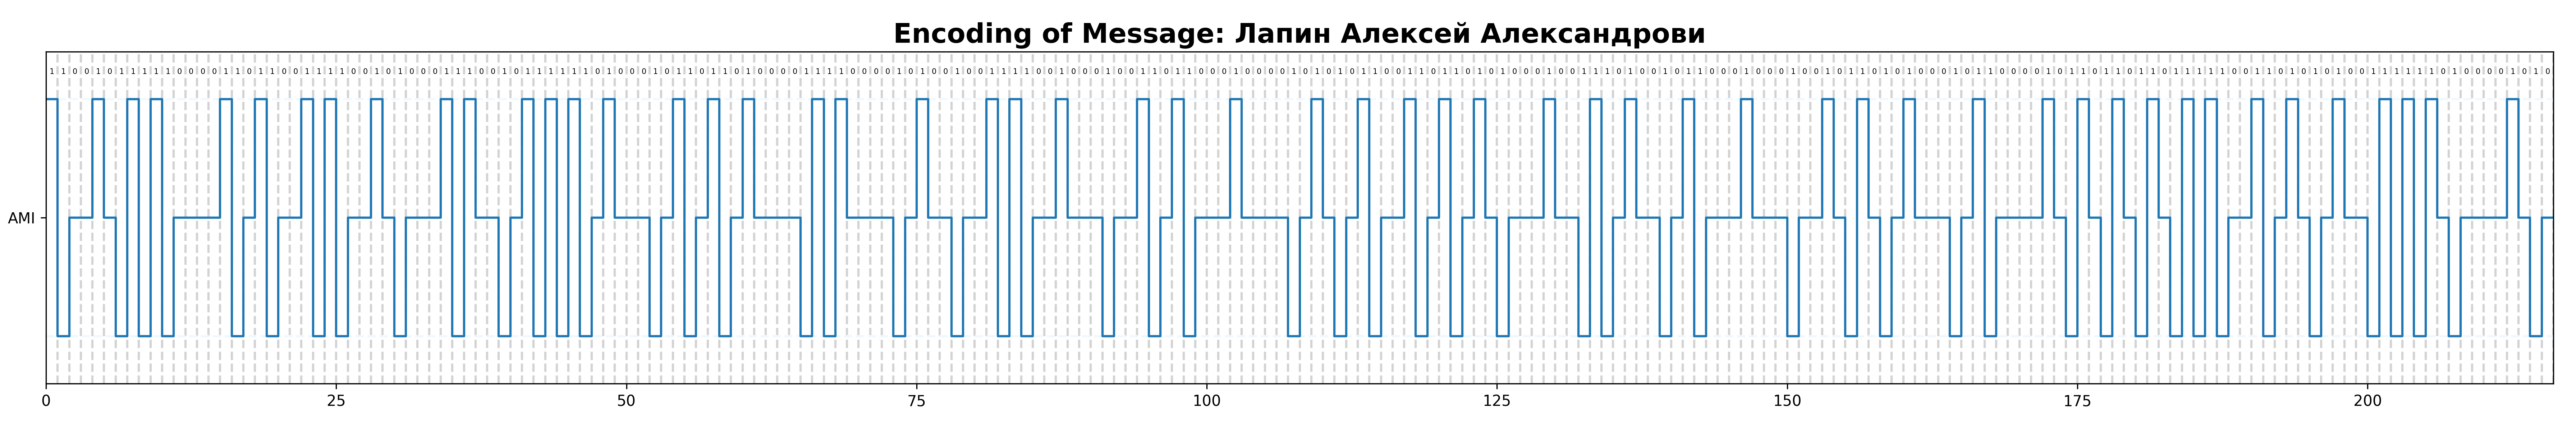
\includegraphics[width=\textwidth]{image/encoding_3-1.png}
    \caption{Скремблирование AMI кода}
\end{figure}

Верхняя граница частот: $f_{\text{в}} = \frac{C}{2} = 50~ \text{МГц}$

Нижняя граница частот: $f_{\text{н}} = \frac{f_0}{4} = 12.5 ~ \text{МГц}$

Средняя частота: $f_{\text{ср}} = \frac{140\cdot f_0 + 14\cdot 2\cdot \frac{f_0}{2} + 8\cdot3 \cdot \frac{f_0}{3} + 6 \cdot 4 \cdot\frac{f_0}{4}}{216} \approx 38.89~\text{МГц}$

Середина спектра: $f_{1/2} = \frac{f_{\text{в}} + f_{\text{н}}}{2} = \frac{50 + 12.5}{2} = 31.25~\text{МГц}$

Спектр сигнала: $S = f_{\text{в}} - f_{\text{н}} = 50 - 12.5 = 37.5~\text{МГц}$

Полоса пропускания: $F = 38~ \text{МГц}$

Сравнивая с AMI кодом в этапе 2, можно сказать, что спектр сигнала немного уменьшился. Также мы уменьшили постоянную состовляющую.
\subsection{Этап 5. Сравнительный анализ результатов кодирования}

\begin{figure}[H]
    \centering
    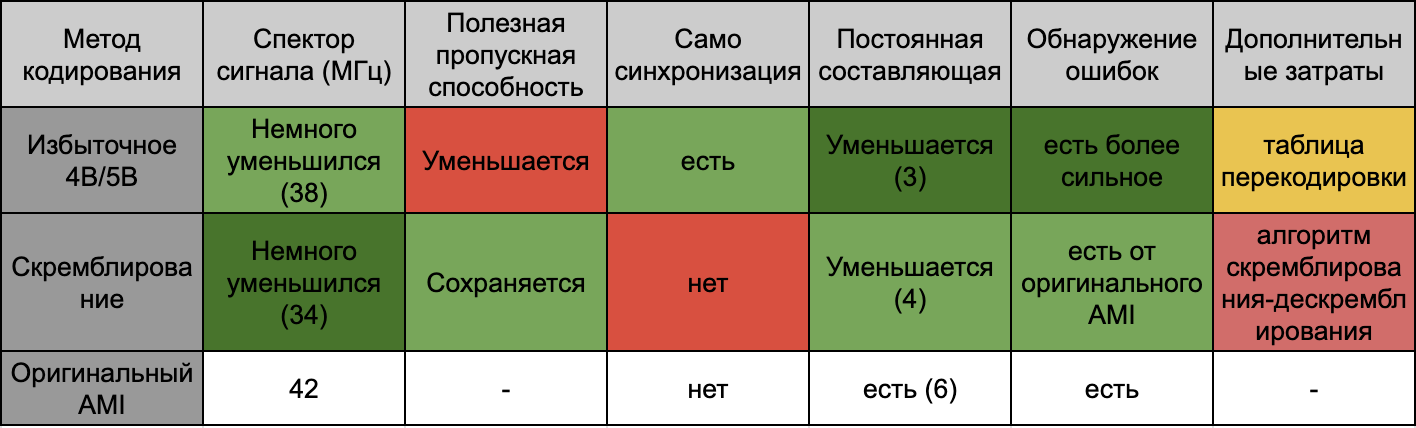
\includegraphics[width=\textwidth]{image/table2.png}
    \caption{Сравнительная таблица результатов кодирования}
\end{figure}

В результате мы видим, что каждый из методов логического кодирования обладает своими плюсами и минусами.

В избыточном кодировании мы уменьшаем спектр сигнала, получаем свойство самосинхронизации, и обнаружение ошибок за счет запрещенных комбинаций единиц и нулей (16 комбинаций в 4B/5B). Также реализация является довольно простой (таблица перекодировки). Но у нас уменьшается полезная пропускная способность из-за добавления дополнительных битов. 

В скремблировании у нас иногда может уменьшаться спектр сигнала, также у нас сохраняется пропускная способность и уменьшается постоянная состовляющая. Но у нас нет свойства самосинхронизации и обнаружения ошибок только на последовательные единицы от оригинального AMI.
Кроме того реализация скремблирования требует больших затрат, чем в избыточном кодировании. 

\section{Часть 2. Передача кодированного сообщения по каналу связи}
\begin{figure}[H]
    \centering
    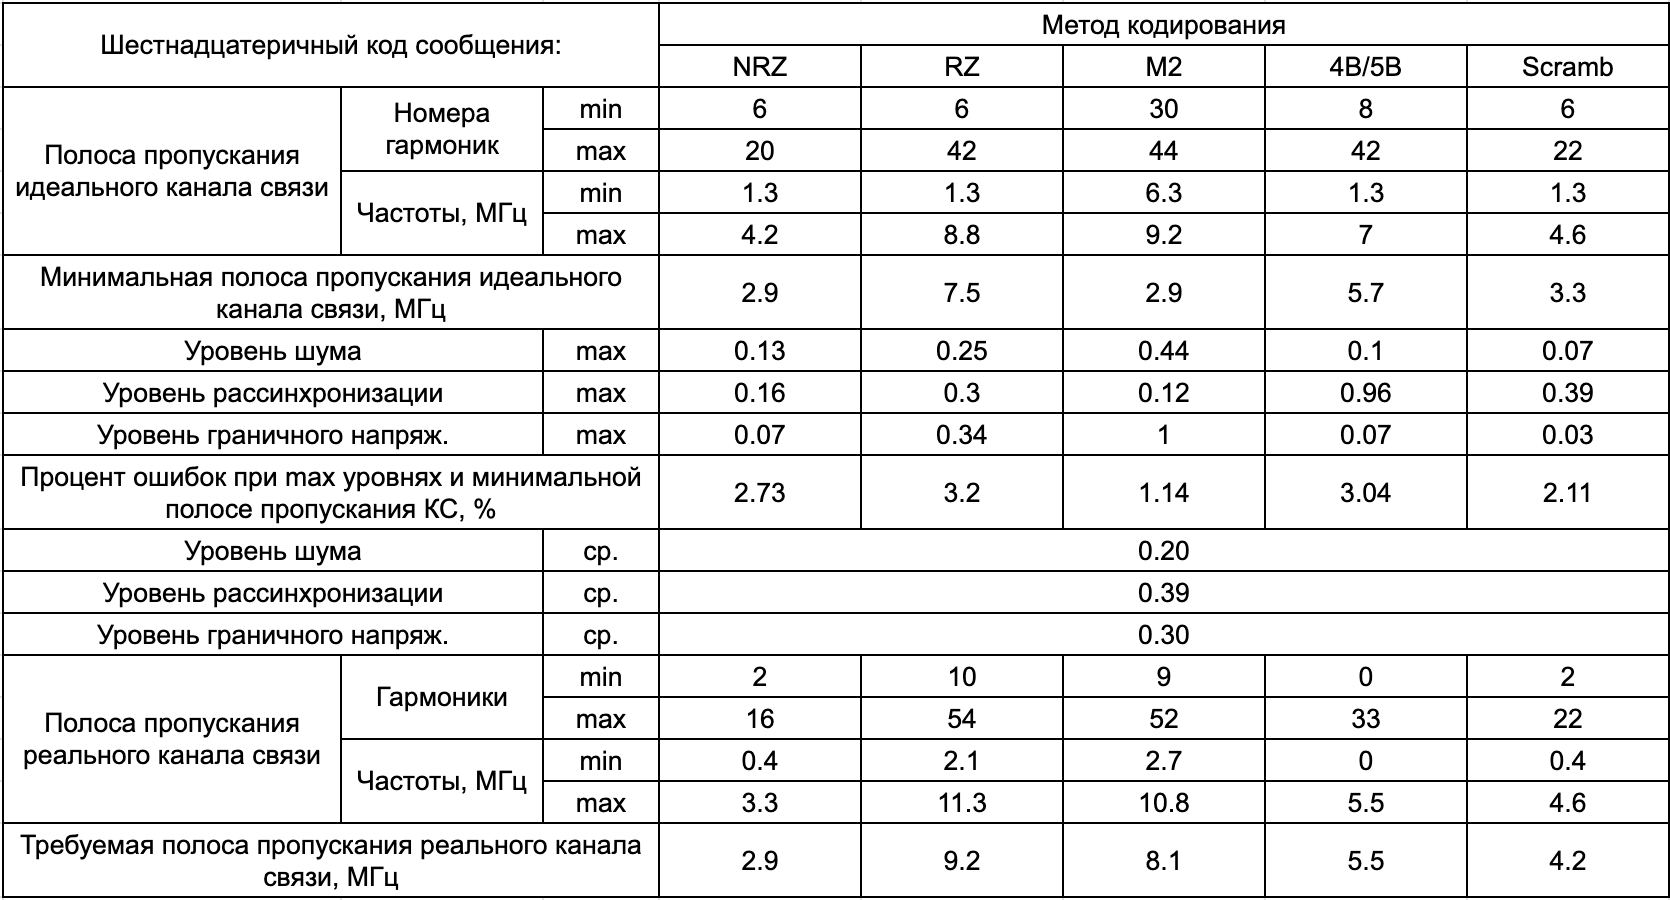
\includegraphics[width=\textwidth]{image/table3.png}
\end{figure}

Вывод:
Для данного сообщения и помех в канале связи лучше всего подходит NRZ код, так как у него наименьшая необходимая полоса пропускания. Но у него довольно скомные результаты в противодействии помехам.

В противодействии шуму и граничному напряжению лучше всего себя показал M2 код, но за это приходится платить довольно широкой полосой пропускания.

С рассинхронизацей лучше всех справился 4B/5B код, также у него средняя величина полосы пропускания.

Скремблирование уступает 4B/5B коду по помехоустойчивости, но имеет меньщую полосу пропускания. 

RZ код уступает M2 по всем показателям и обладает самой широкой полосой пропускания.




\end{document}